\begin{tikzpicture}[scale=0.9,transform shape] 
	\onslide<2->{ \node[] (input_taj) 
		{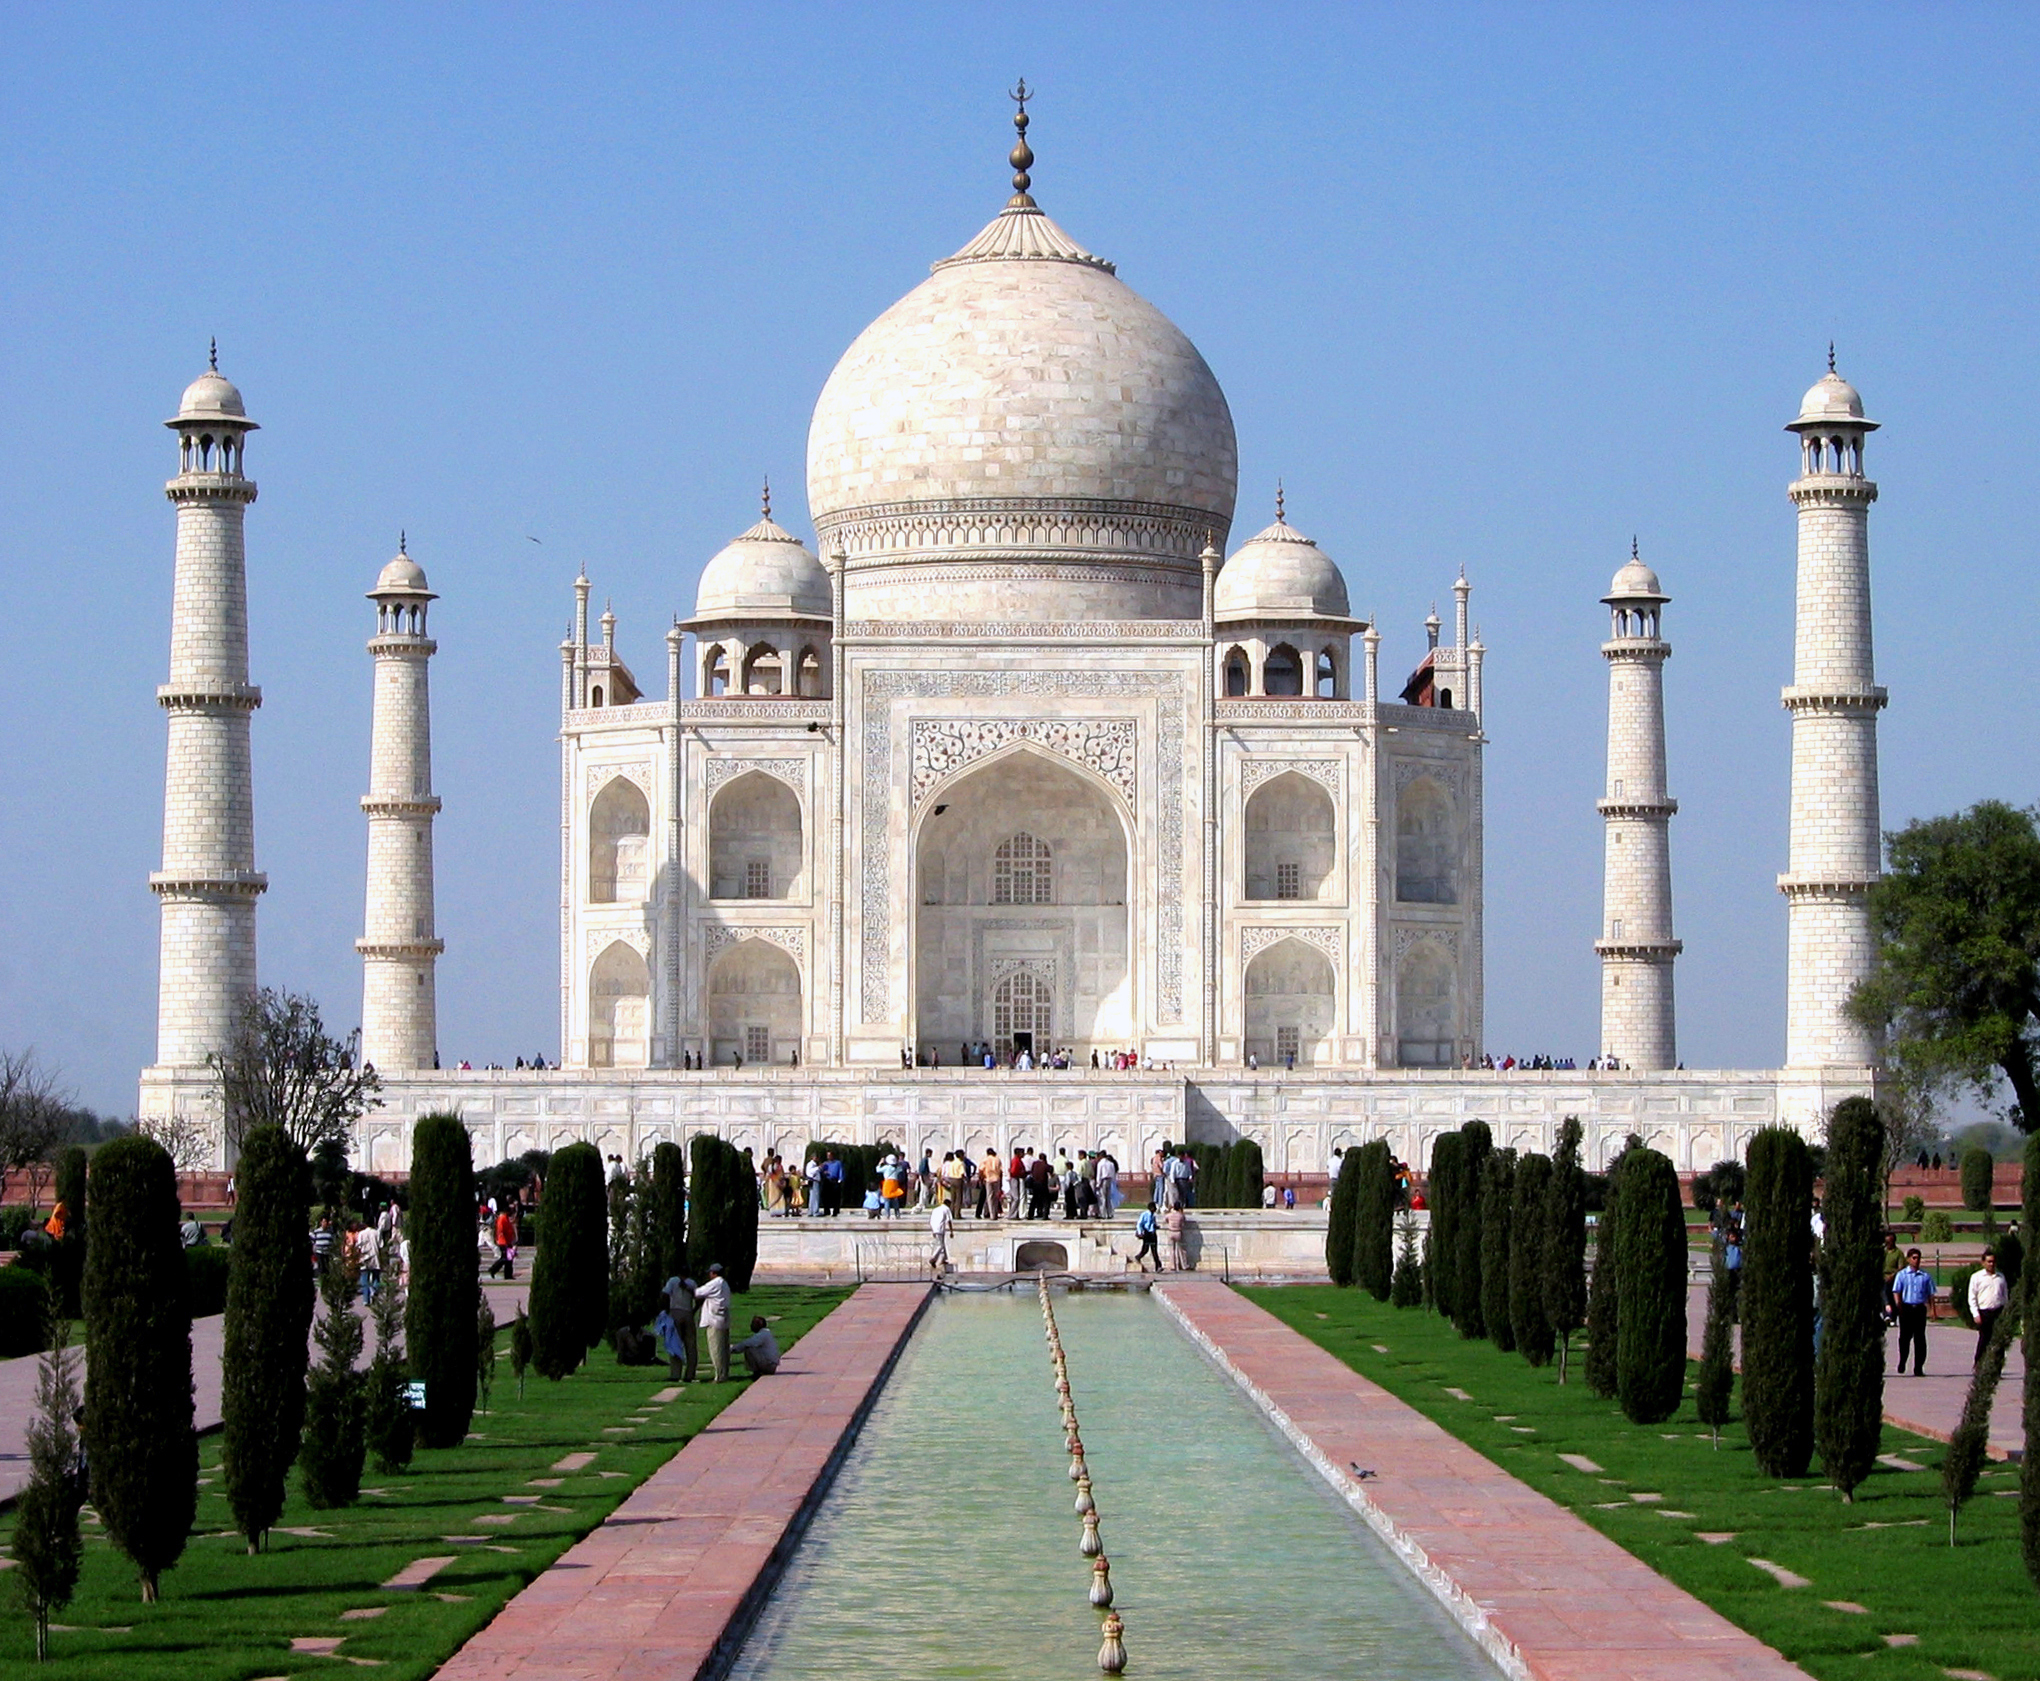
\includegraphics[width=20mm,height=17mm,scale=0.7]{images/taj_mahal.jpg}};
	}
	\onslide<2->{  \node (raw) at ($(input_taj) + (4,0)$)  { 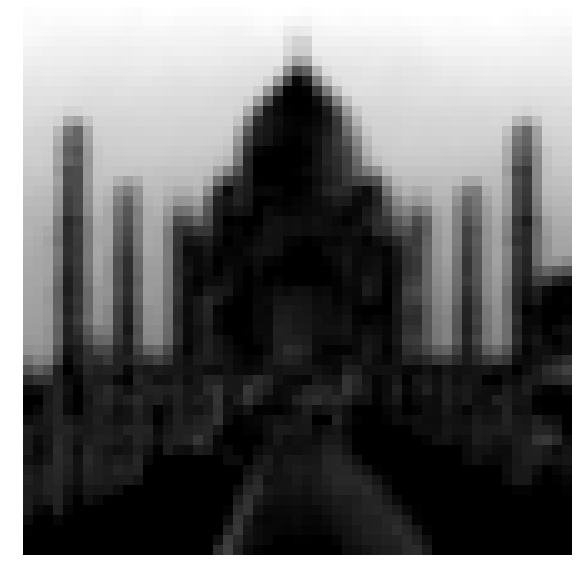
\includegraphics[width=20mm,height=17mm,scale=0.7]{images/convo1.png}};
		\node [below of = raw,anchor=north] (edge)  { \resizebox{25mm}{8mm}{ \begin{tabular}{ccccc}
			-1.21358689e-03  & 3.23652686e-03 & $\cdots$ & $\cdots$ & -2.06615720e-02\\ 
			-1.52757822e-03  & 2.36130832e-03 & $\cdots$ & $\cdots$ & -1.19824838e-02\\ 
			$\vdots$ & $\vdots$ &  &  & $\vdots$\\ 
			$\vdots$ & $\vdots$ &  &  & $\vdots$\\ 
			-8.25322699e-04 & -5.14897937e-03 &  $\cdots$ & $\cdots$ &-9.90395527e-03 \\
			\end{tabular} }};
		%\node[above of= raw,node distance=1.2cm ] (features)  {\footnotesize{Features}};
		\draw[->,thick] (input_taj) -- (raw) ;

	}
	\onslide<2->{\node(output_taj) at ($(input_taj) + (9,0)$) {car, bus, \textcolor{blue}{monument}, flower};
		\draw[->,thick] (raw) -- (output_taj) ;}
	
	\onslide<3->{\node [] (edge1) at ($(edge) + (5,0)$){{\textcolor{red}{Learn these weights}}};
		\draw [->, thick] (edge1) -- (edge);
	}

\end{tikzpicture}